\chapter{Grundlagen}
\thispagestyle{fancy}

\section{Bandstruktur von Gruppe-III Nitriden}
\begin{figure}[!htb]
    \centering
    \begin{minipage}[t]{\linewidth}
        \centering
        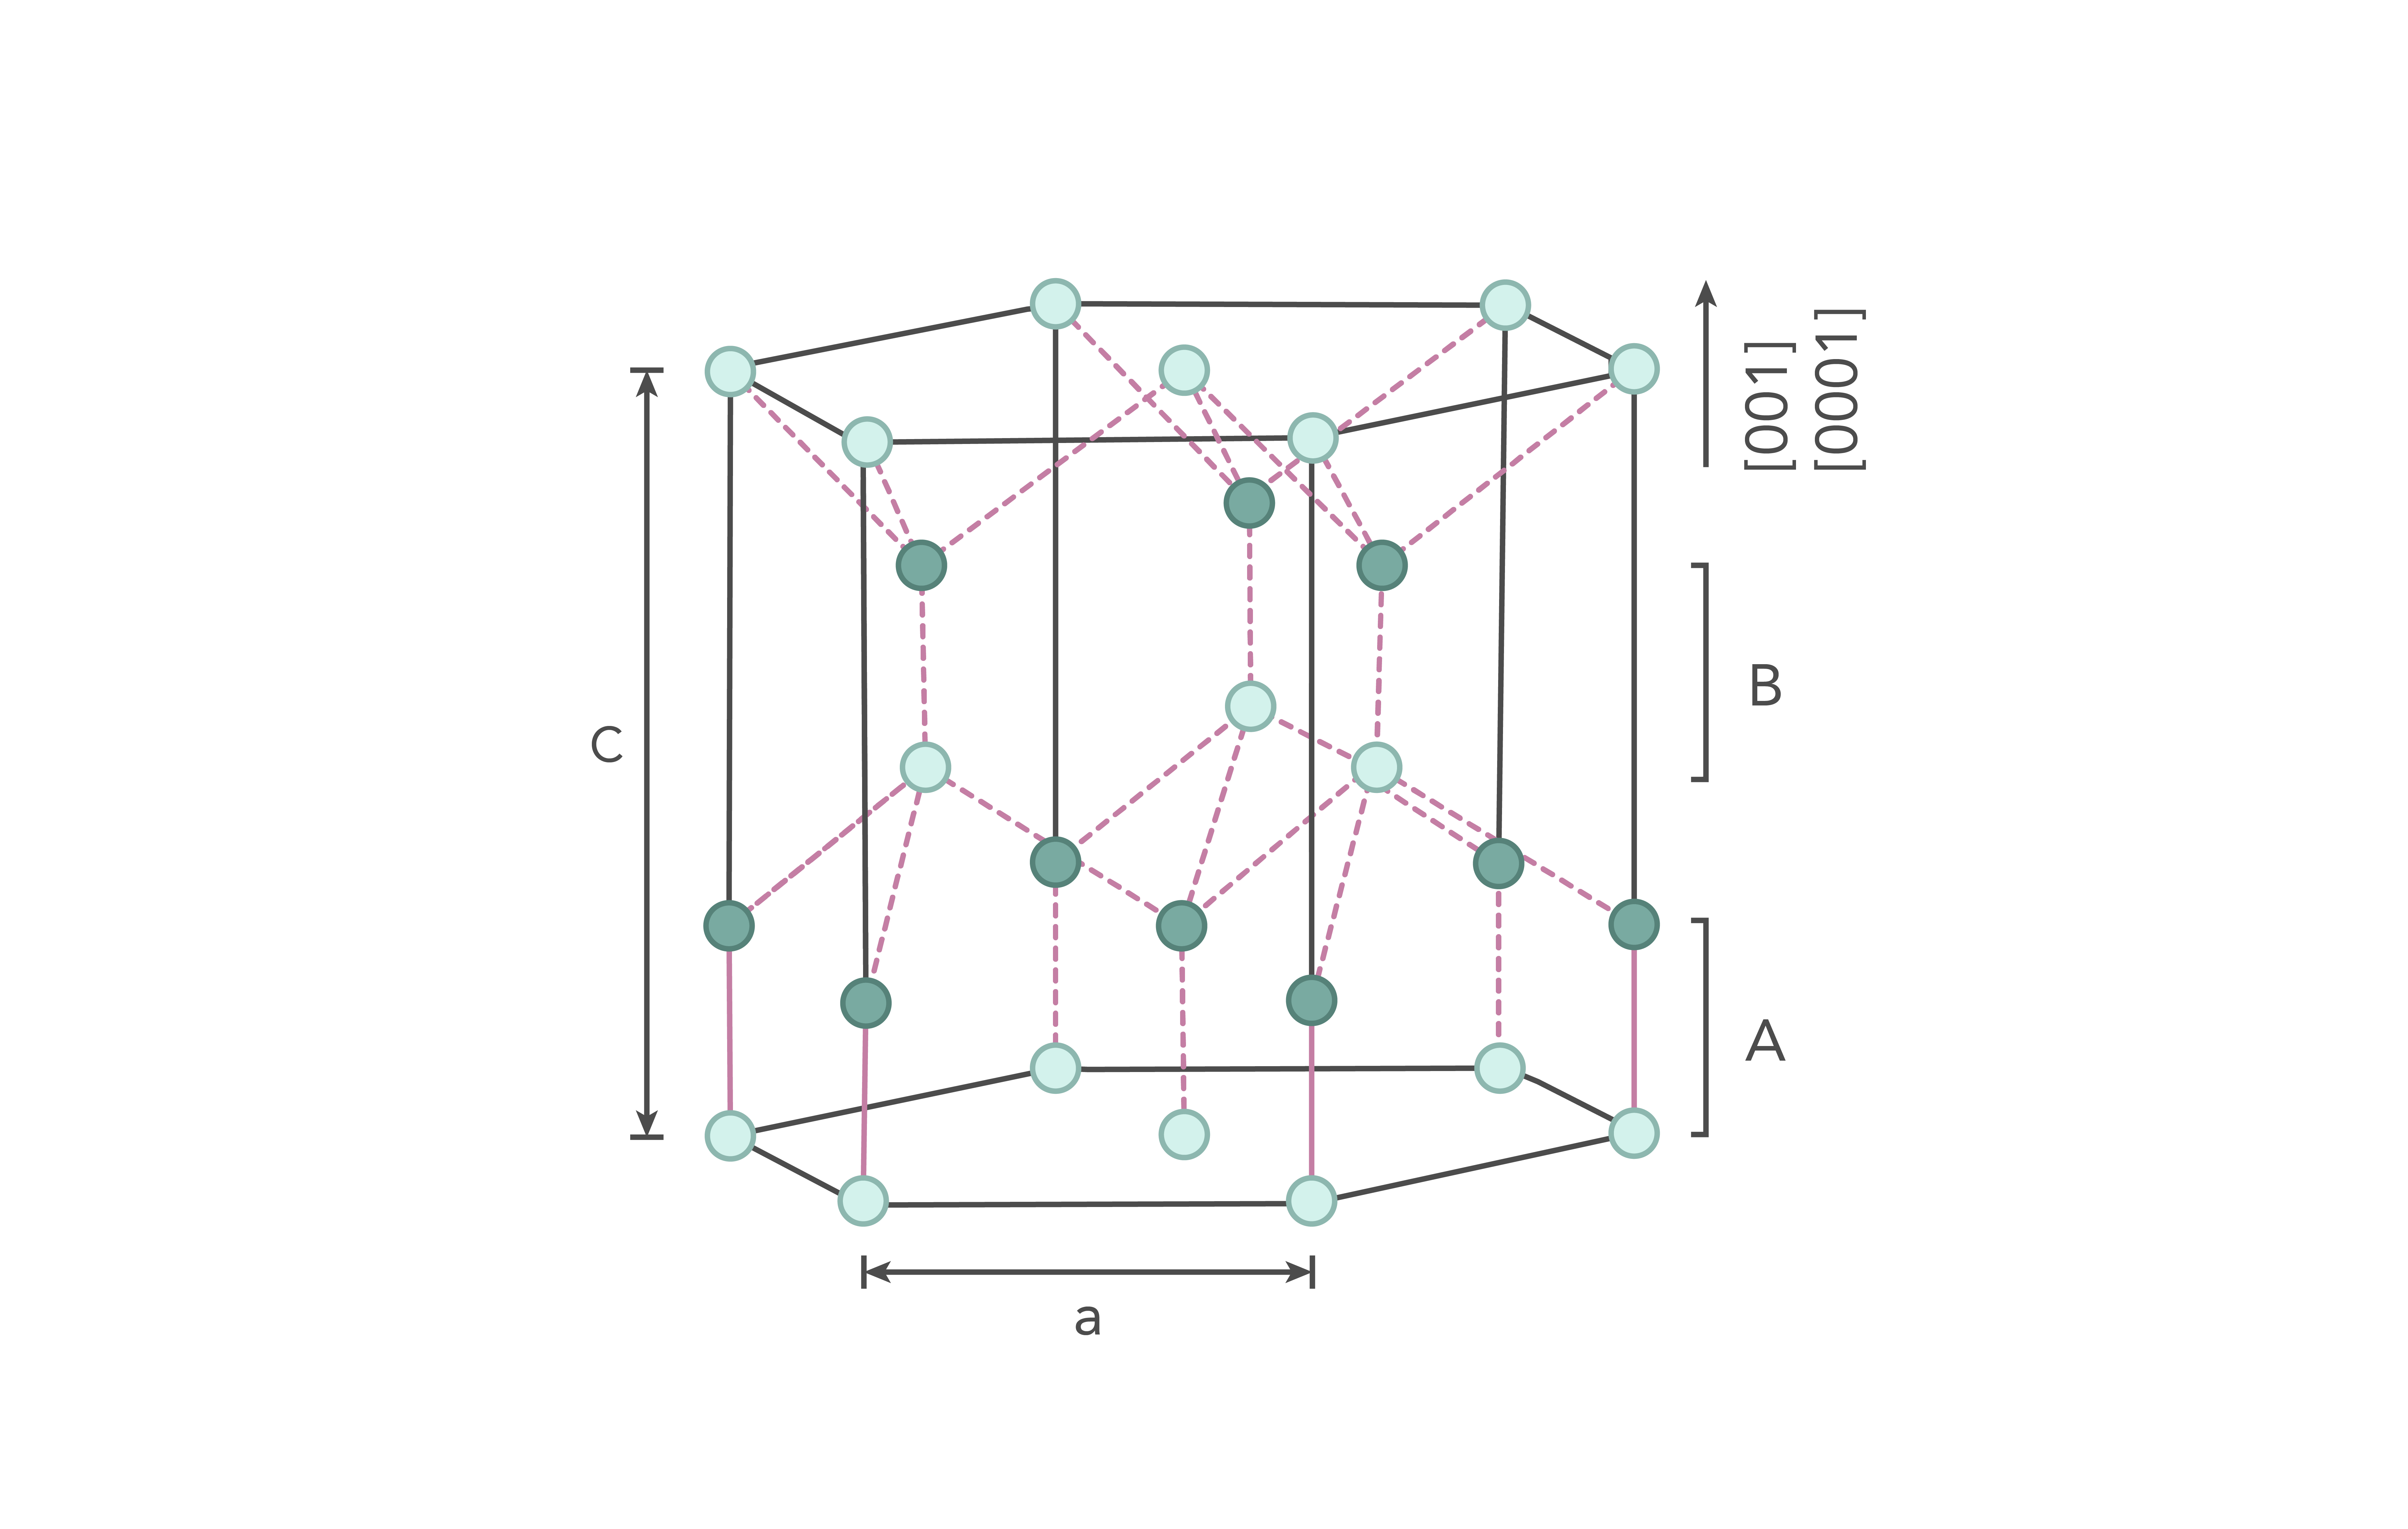
\includegraphics[width=0.7\linewidth]{Bilder/Wurtzite.png}
        \caption{Einheitzelle der hexagonale Wurtzitstruktur. Die schwarzen Kreise stellen die Position der Stickstoffatome im Gitter dar. Die Gitterposition der Gruppe-III-Metallatome stellen sind als graue Kreise dargestellt. A und B bezeichnen die Stapelebene.  }
        \label{fig:wurtz}
    \end{minipage}% <- sonst wird hier ein Leerzeichen eingefügt
\end{figure}
\vspace{1cm}
\raggedright


Die wichtige Gruppe der III-Nitridhalbleiter setzt sich aus den Metallen
der dritten Hauptgruppe Aluminium (Al), Gallium (Ga) und Indium (In) zusammen.
Anschaulich bedeutet dies, dass ausgehend von der hexagonal dichtesten Kugelpackung in Doppellagen, die Gruppe-III-Metallen und Stickstoff (N) sich entlang der c-Achse in der Abfolge A-B-A-B anordnen~\cite{buchc} wie in Abb. [\ref{fig:wurtz}] dargestellt ist. 
Diese kristallisieren bevorzugt in der hexagonalen Wurtzitstruktur Abb. [\ref{fig:wurtz}].
Der Schwerpunkt dieser Arbeit liegt auf dem AlGaN-Materialsystem mit hohen Al-Konzentration. Das Mischverhältnis bestimmt hierbei die Bandlückenergie des Verbindungshalbleiters. Durch die unterschiedlichen Bandlückenergien von Aluminium mit $6,03 \thinspace eV$ ~\cite{fenaln} und GaN mit $3,4 \thinspace eV$ ~\cite{pipr} eignet sich AlGaN besonders für die Emission im Wellenlängenbereich von UV-A bis UV-C. 
Die Bandlückenenergie von AlGaN lässt sich durch Interpolation der binären Energien von GaN und AlN in Abhängigkeit des Kompositionsverhältnisses x berechnen, wobei ein zusätzlicher Bowing-Parameter für die nichtlineare Abweichung hinzugefügt wird. 
%
\begin{equation}
    E_{Al_{x}Ga{1-x}N} = E_{AlN} \cdot x + E_{GaN} \cdot (1-x) - b_{AlGaN} \cdot x \cdot (1-x) 
\end{equation}
%
Die Gruppe um Lee et al. gibt nach Auswertung der in der Literatur vorkommenden unterschiedlichen Bowing-Parameter für $Al_{x}Ga_{1-x}N$ einen Wert von $b_{AlGaN} = 0,62\thinspace(\pm \thinspace 0,45)\thinspace eV$ und geben weiter an, das hohe Wachstumstemperaturen zu großen Bowing-Parametern führen ~\cite{doi:10.1063/1.123339}.
Vurgaftman et al. empfiehlen unter Berücksichtigung weiterer Veröffentlichungen für $b_{AlGaN} =  0,7 \thinspace eV$ 
%
\newpage
\section{Polarisationsfeld und QCSE in III/V Halbleitern}

Aufgrund der fehlenden Inversionssymmetrie und stark unterschiedlichen Elektronegativitäten des Stickstoffs und der entsprechenden Gruppe III-Metalle bilden sich Polarisationsfelder aus, die entlang der auf der Basalebende stehenden c-Achse verlaufen. Hier unterscheidet man zwischen zwei Arten von Polarisationsfeldern, die spontane Polarisation $ \vec{P}^{sp} $ und die piezoelektrische Polarisation $ \vec{P}^{pz} $.
\newline\newline
Die spontane Polarisation entsteht durch Dipolmomente im Kristall die sich aufgrund von ungleichen Bindungslängen nicht komplett aufheben. Ursprung der 
Dipolmomente im AlGaN sind die unterschiedlichen Elektronegativitäten zwischen den Gruppe III-V Elementen und bedingt durch die angestrebte Minimierung der Gesamtenergie, kommt es zur Abweichung vom idealen Tetraederwinkel von $109,5^{\circ}$~\cite{ambacher2002}.
%
\begin{figure}[htb]
    \centering
    \begin{minipage}[t]{0.7\linewidth}
        \centering
        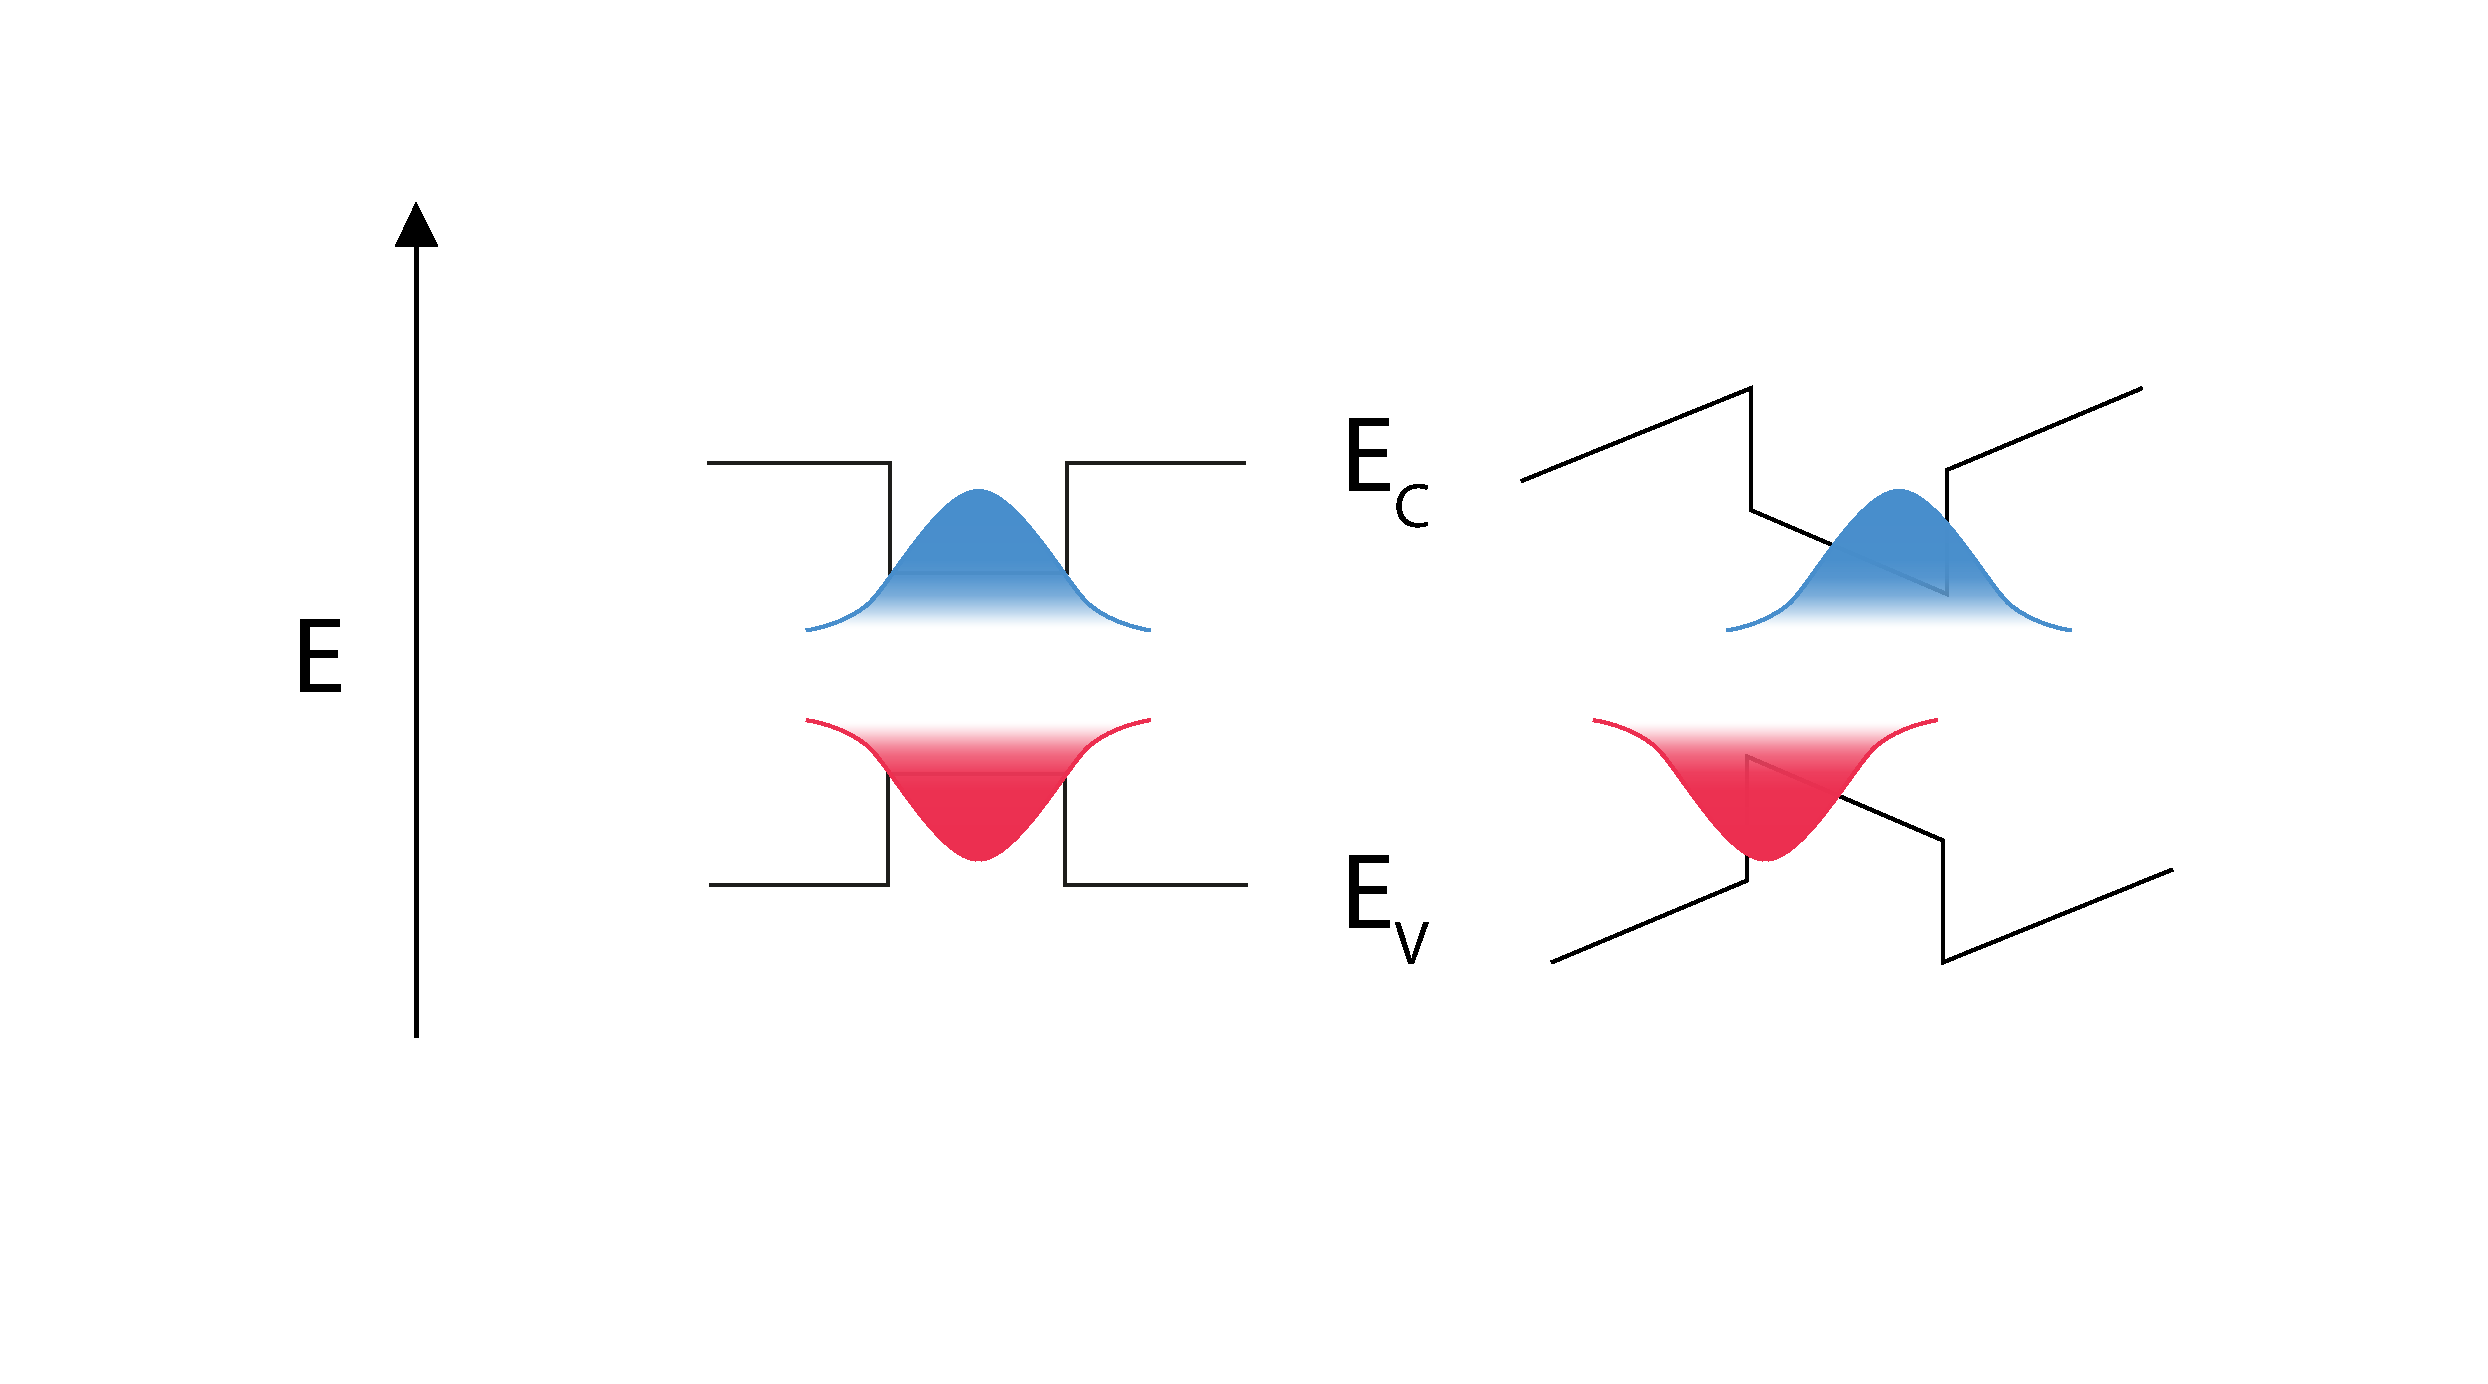
\includegraphics[width=\linewidth]{Bilder/QCSE.pdf}
        \caption{Einluss der spontanen und piezolektrischen Polarisation auf Valenz- und Leitungsband einer Quantenfilm-Heterostruktur. Die Aufenthaltswahrscheinlichkeiten von Elektronen und Löchern werden verschoben.}
        \label{fig:qcse}
    \end{minipage}% <- sonst wird hier ein Leerzeichen eingefügt
\end{figure}
\vspace{1cm}
\raggedright
\newpage
Die Ursache für die piezoelektrische Polarisation sind die Verspannungen zwischen den in (0001)-Richtung gewachsenen Schichten welche durch die unterschiedlichen thermischen Ausdehnungskoeffizienten und die Gitterfehlanpassung beim pseudomorphen Wachstum entstehen. Sie wird berechnet nach
%
\begin{equation}
    \vec{P}^{pz} = e \cdot \epsilon
\end{equation}
%
mit Dehnung $\epsilon$ und dem piezolektrischen Tensor $\vec{e}$ (Tensor dritter Stufe).
\newline
In Heterostrukturen führt der Wechsel der Gesamtpolarisation $\vec{P}^{gesamt} = \vec{P}^{pz} + \vec{P}^{sp}$ zwsichen den einzelnen Schichten zur Ansammlung von Ladungsträgern an den Grenzflächen. Dies ist insbesondere für die Effizienz von Leucht-und Laserdioden von Nachteil. Denn in diesen erzeugen die induzierten Grenzflächenladungen ein elektrisches Feld, das zur einer Bandverbiegung führt (siehe Abb.[\ref{fig:qcse}]). Mit dem Einfluss der Polarisation sammeln sich die Elektronen und Löcher im Quantenfilm somit auf gegenüberliegenden Seiten. Dies führt dazu, dass der räumliche Überlapp der Wellenfunktionen von Elektronen und Löchern abnimmt. Durch das verringerte Überlappintegral der Wellenfunktionen sinkt nach Fermis Goldener Regel auch die strahlende Rekombinationsrate. Dieser Effekt wird als "Quantum Confined Stark Effekt" (QCSE) bezeichnet. Des Weiteren sinkt die effektive Bandlücke und ist im Spektrum durch eine Rotverschiebung der Emission zu erkennen. Bei hohen Ladungsträgerdichten im Quantenfilm kommt es zur Abschirmung (engl. screening) der Grenzflächenladungen die die Auswirkungen des Effektes abschwächen.
